\begin{figure}[tp!]
	\center
	\begin{subfigure}{0.24\textwidth}
		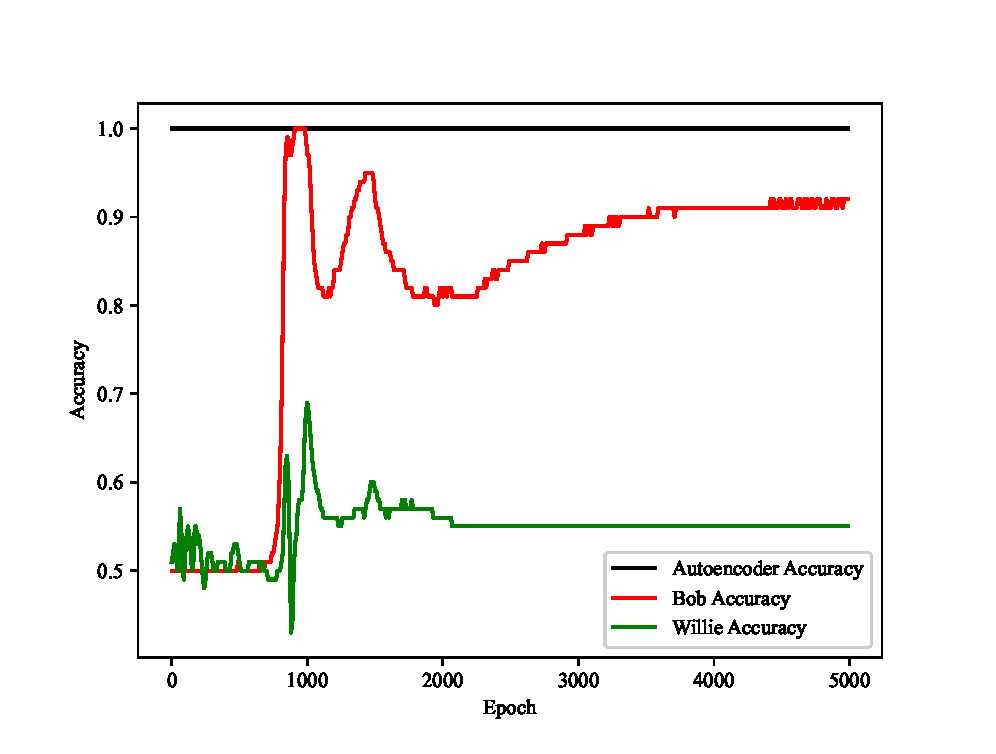
\includegraphics[width=\linewidth]{figs/training_progress_awgn}
		\caption{AWGN channel}
	\end{subfigure}
	\hfill
	\begin{subfigure}{0.24\textwidth}
		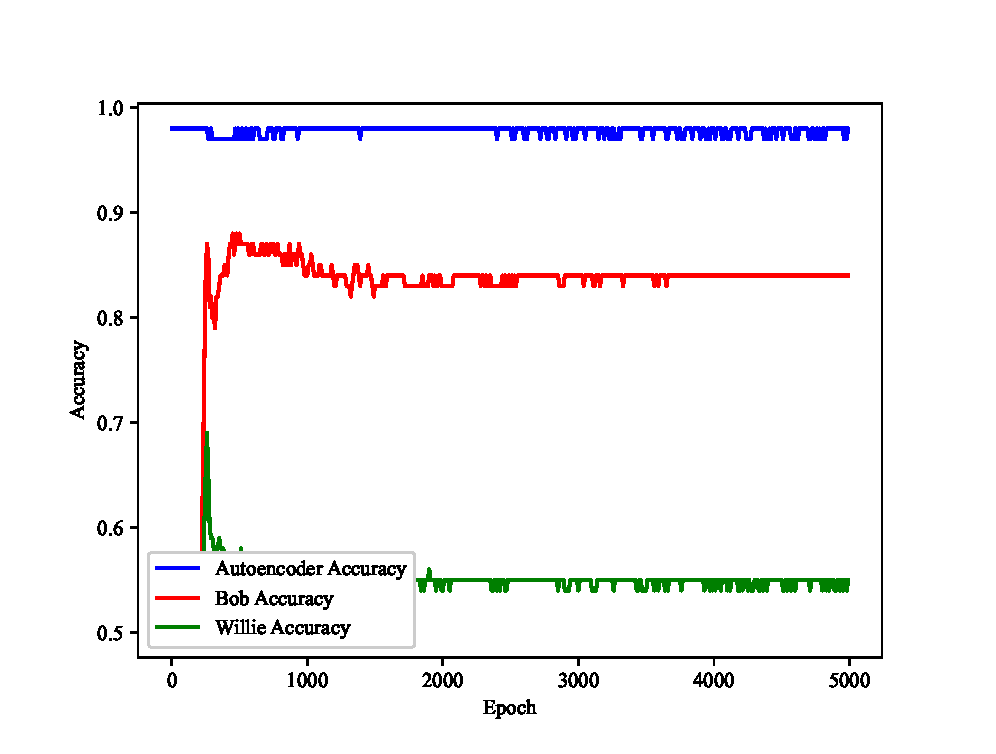
\includegraphics[width=\linewidth]{figs/training_progress_rayleigh}
		\caption{Rayleigh fading channel}	
	\end{subfigure}
	\caption{Covert models' accuracies evaluation during training progress}
	\label{fig:traning_progress}
\end{figure}
\section{Experiments and Evaluation}
\label{s:eval}
Before implementing the covert models, we implemented an autoencoder communication network for the normal communication between UserRX and UserTX. The functionality and architectural design of this model is already described in the previous section. Based on the notation used in \cite{o2017introduction}, an \(Autoencoder (n, k)\) is a neural network communication model that sends \(k\) bits of data in \(n\) channel uses. We chose these two numbers of channel uses \(n\) and the binary message of size \(k\) to be 8 and 4, respectively. These numbers are chosen this way so that we could evaluate the performance of our trained autoencoder model with the results given on \cite{o2017introduction}. Nevertheless, our covert model works independent of these parameters and can be used for any autoencoder communication setup. In order to train our autoencoder model, we generate two datasets of train and test by generating random binary messages \(s\) of size \(k\). The training set contains 8192 random binary messages while this number is 51200 for the test set. We intentionally created a much larger data set for testing to make sure that each symbol \(y\) undergoes various channel distortions while evaluating the model's performance. We set the learning rate to 0.001 and optimized the model using the Adam optimizer \cite{kingma2014adam}. We chose the batch size to be 64 and trained the model for 100 epochs. For the channel configuration, we chose fixed signal to noise ratio (SNR) values during the training. The SNR value for the AWGN channel is set to 4dB, and we give a higher SNR value of 16dB to the Rayleigh fading channel due to the channel complexity. Figure (\ref{fig:autoencoder_bler}) shows the performance of our trained normal communication models in terms of block error rate (BLER) for a range of SNR values under AWGN and Rayleigh fading channel conditions.\\
\begin{figure}[bp!]
	\center
	\begin{subfigure}{0.35\textwidth}
		\includegraphics[width=\linewidth]{figs/autoencoder_bler_awgn}
		\caption{AWGN channel}
	\end{subfigure}
	\begin{subfigure}{0.35\textwidth}
		\includegraphics[width=\linewidth]{figs/autoencoder_bler_rayleigh}
		\caption{Rayleigh fading channel}	
	\end{subfigure}
	\caption{Trained Autoencoder's BLER over a range of SNR values}
	\label{fig:autoencoder_bler}
\end{figure}
\begin{figure*}[th!]
	\begin{subfigure}{0.3\textwidth}
		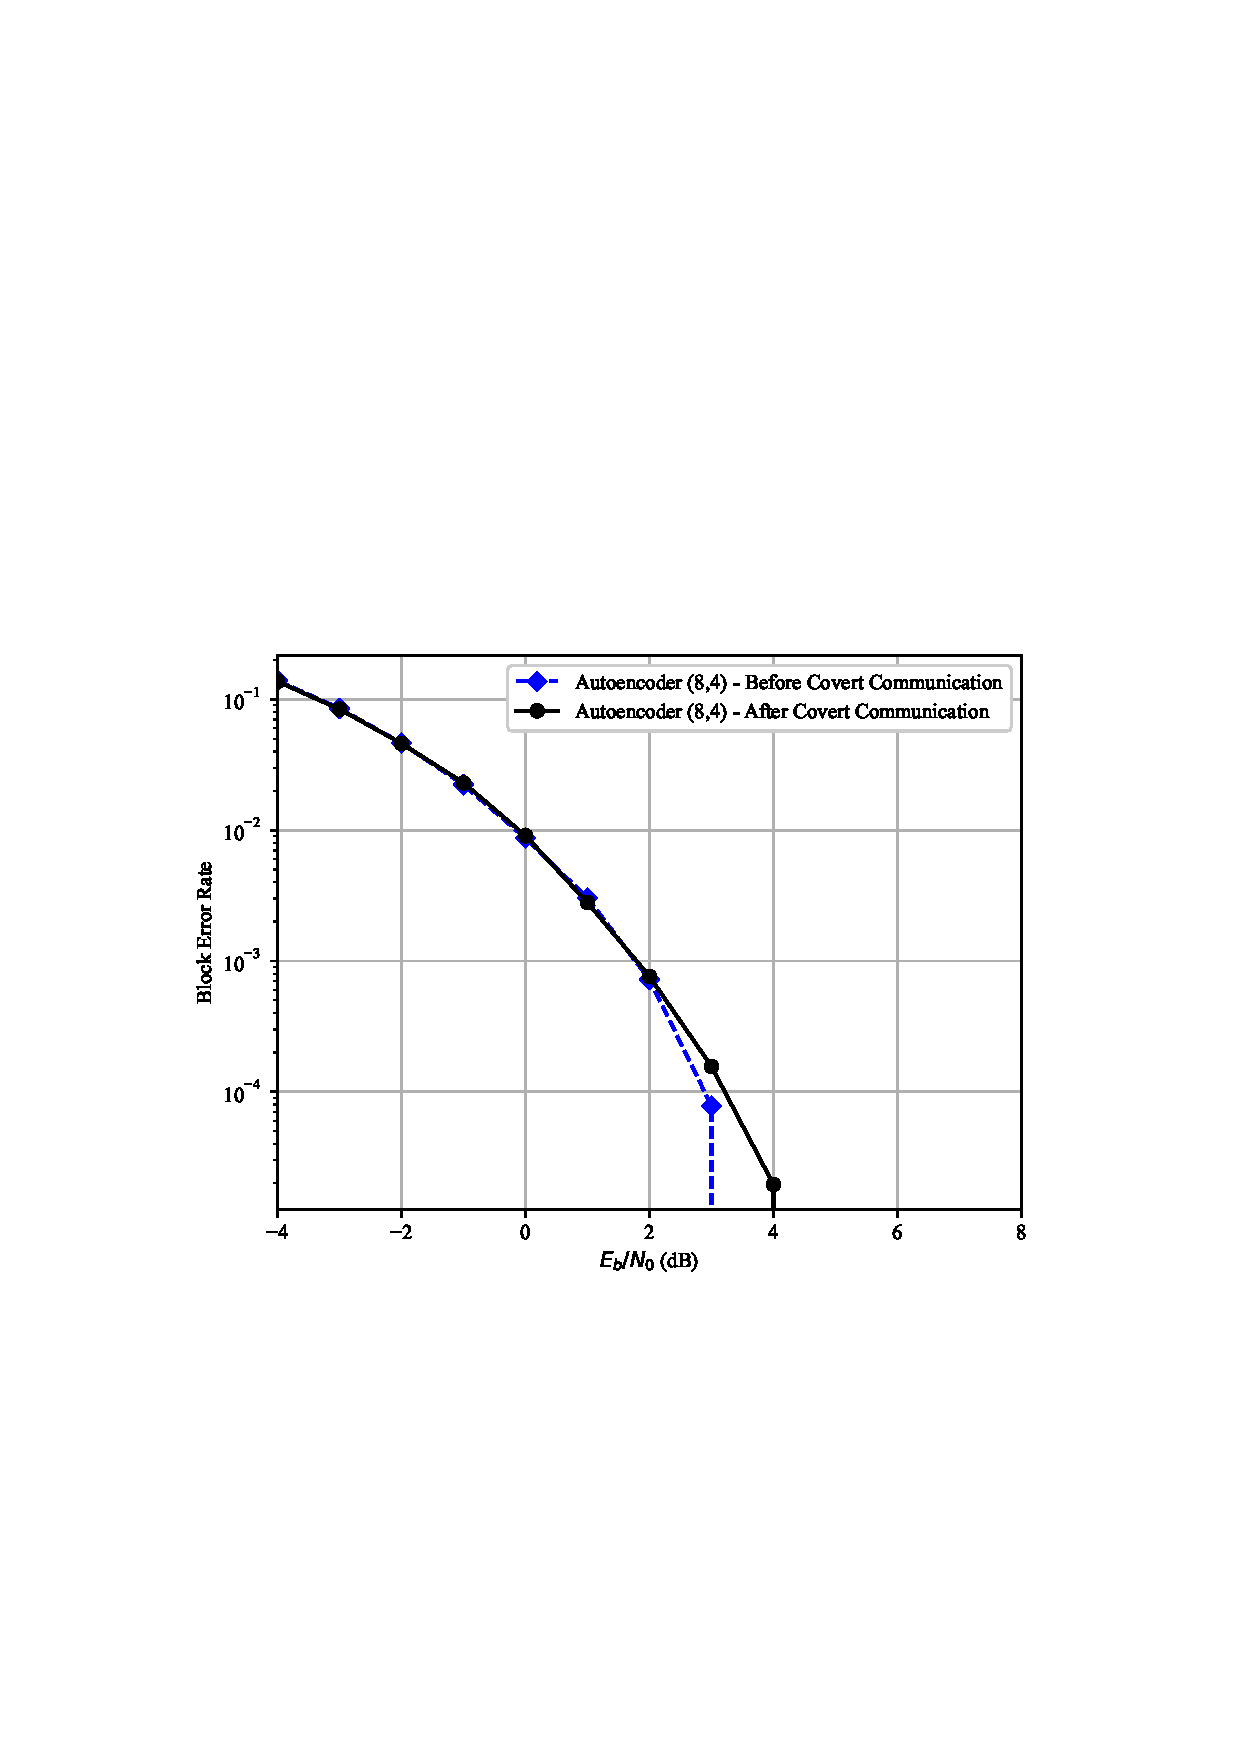
\includegraphics[width=\linewidth]{figs/covert_autoencoder_bler_awgn}
		\caption{Autoencoder's BLER}
		\label{fig:awgn_resutls_ae}
	\end{subfigure}
	\hspace*{\fill}
	\begin{subfigure}{0.3\textwidth}
		\includegraphics[width=\linewidth]{figs/bob_bler_awgn}
		\caption{Bob's BLER}	
		\label{fig:awgn_resutls_bob}
	\end{subfigure}
	\hspace*{\fill}
	\begin{subfigure}{0.3\textwidth}
		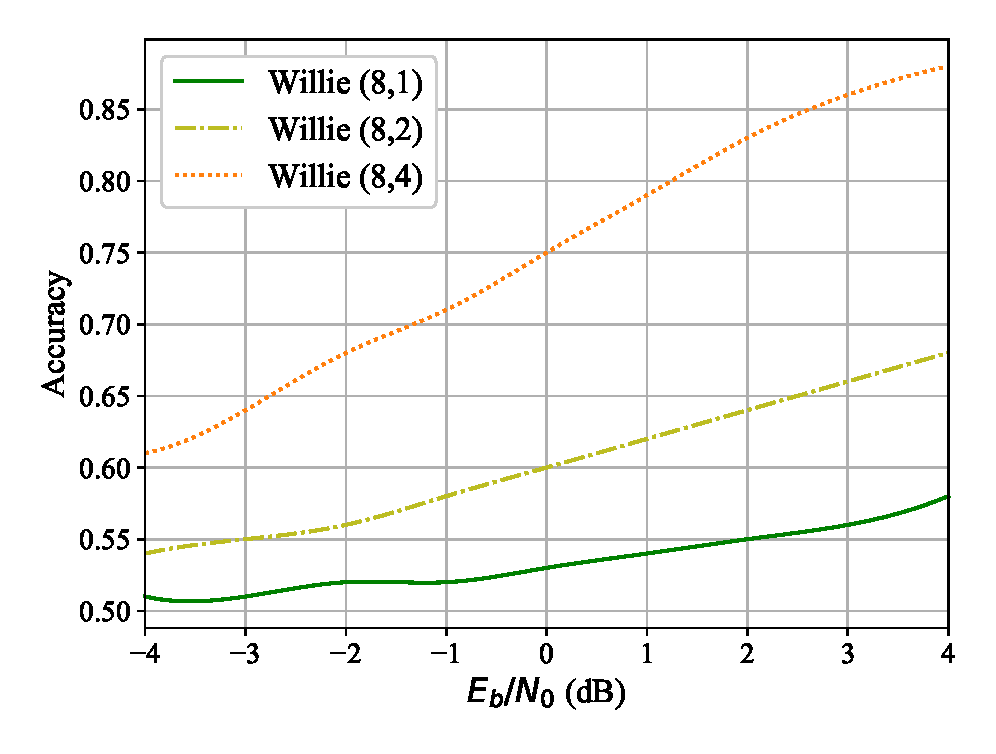
\includegraphics[width=\linewidth]{figs/willie_accuracy_awgn}
		\caption{Willie's accuracy}	
		\label{fig:awgn_resutls_willie}
	\end{subfigure}
	\caption{Trained covert models' performance over AWGN channel for different covert data rates.}
	\label{fig:awgn_results}
\end{figure*}
\begin{figure*}[tp!]
	\begin{subfigure}{0.3\textwidth}
		\includegraphics[width=\linewidth]{figs/covert_autoencoder_bler_rayleigh}
		\caption{Autoencoder's BLER}
		\label{fig:rayleigh_resutls_ae}
	\end{subfigure}
	\hspace*{\fill}
	\begin{subfigure}{0.3\textwidth}
		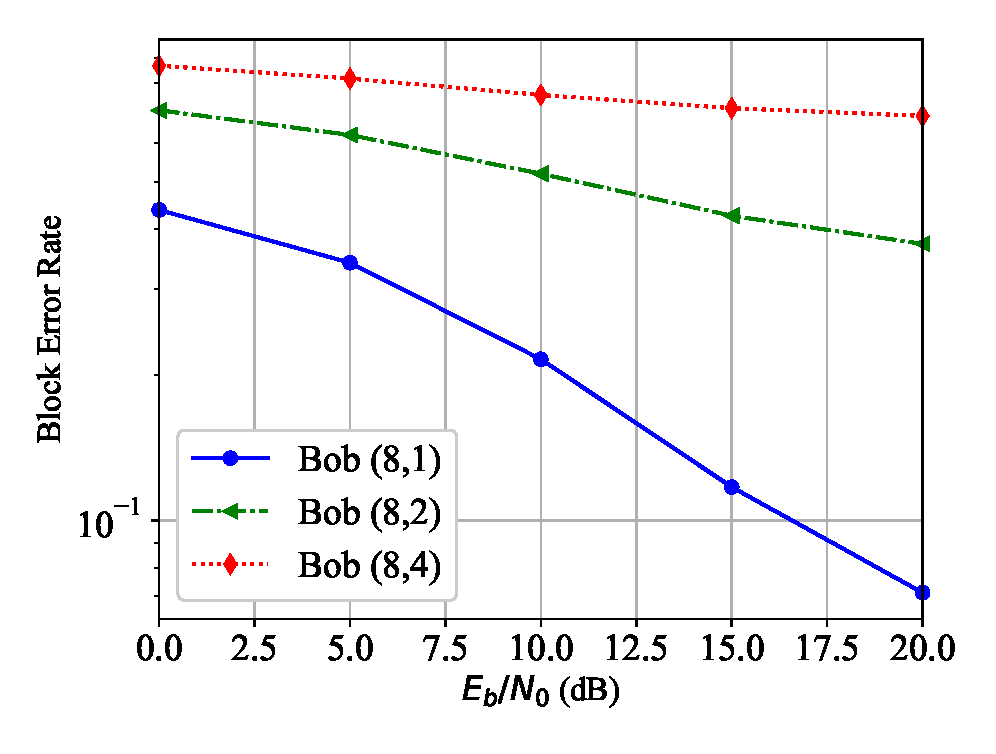
\includegraphics[width=\linewidth]{figs/bob_bler_rayleigh}
		\caption{Bob's BLER}
		\label{fig:rayleigh_resutls_bob}	
	\end{subfigure}
	\hspace*{\fill}
	\begin{subfigure}{0.3\textwidth}
		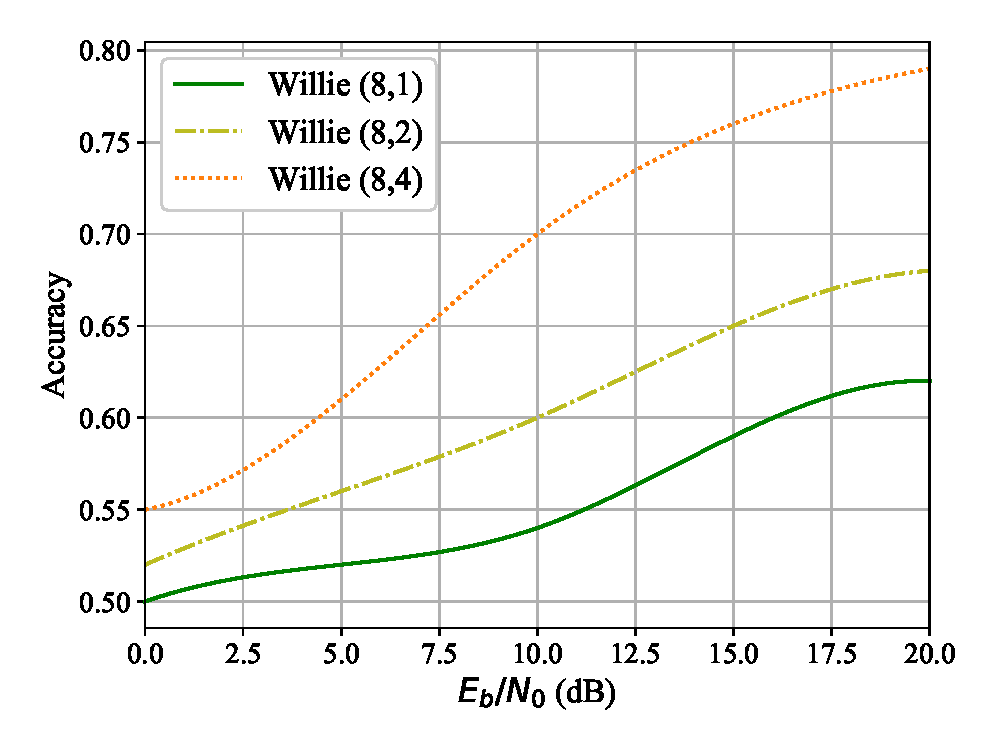
\includegraphics[width=\linewidth]{figs/willie_accuracy_rayleigh}
		\caption{Willie's accuracy}
		\label{fig:rayleigh_resutls_willie}
	\end{subfigure}
	\caption{Trained covert models' performance over Rayleigh fading channel for different covert data rates}
	\label{fig:rayleigh_resutls}
\end{figure*}
As for the covert models, we evaluated the our system's performance on the two different channel models of AWGN and Rayleigh fading. In both settings, we used the same training procedure and network architecture for our covert models. We started our experiment by sending 1 bit of covert data over 8 channel uses and then gradually increased the number of covert bits to see how increasing the covert data rate would effect each component of our covert scheme. The notations \(Alice (n,k)\), \(Bob (n,k))\), and \(Willlie (n,k)\) are used to differentiate models operating on different bit rates and the interpretation of it is just the same as what was explained for the autoencoder model. Since each covert message has to be paired with a normal message, we generated train and test covert messages \(m\) to have the same number of train and test messages as of the autoencoder's. All models are jointly trained for 5000 epochs using Adam optimizer. We start the training with the learning rate of 0.001 and gradually halve the learning rate after every 500 epochs. In each epoch, we first update parameters of Willie's network using (\ref{willie_loss}), then train Alice's network for one step using (\ref{alice_loss}), and eventually optimize Bob's network based on (\ref{bob_loss}). Although we trained our autoencoder network on a fixed SNR value, we found our covert scheme better performs when trained on a range of SNR values. We observed training our models this way, not only helps Alice to better preserve the normal communication's accuracy but also makes Bob to be able decoding covert messages more accurately on lower SNR values. Accordingly, we set the SNR value to be in the range of -2dB to 8dB for the AWGN channel and 10dB to 20dB for the Rayleigh fading channel.
Figure (\ref{fig:traning_progress}) shows the progress of each covert actor's accuracy on the test set during the training process. As the training goes on, Bob gradually learns to decode covert messages \(m\) and establishes a reliable communication with Alice. After a few epochs, when the covert communication begins to take up, signals start to deviate from the distribution they had, causing Willie to better detect covert signals. When Willie's accuracy increases, the term \(\mathcal{L}_{Willie}\) dominates the other two objectives of Alice's loss function in (\ref{alice_loss}). This causes Alice to gradually sacrifice its accuracy for the sake of undetectability. Soon afterwards, the training process reaches a stable point where neither of covert models sees any noticeable improvement in their performance as the training continues. Figures (\ref{fig:awgn_results}) and (\ref{fig:rayleigh_resutls}) show our final results. It also demonstrates how each entity's accuracy of our covert model changes as we increase the covert rate. Expectedly, the covert communication becomes more unreliable, the impact on normal communication increases, and the detection becomes easier as the covert rate increases. In figures (\ref{fig:awgn_resutls_willie}) and (\ref{fig:rayleigh_resutls_willie}) the accuracy of Willie is shown in percentage over a range of SNR values for flagging signals as covert and non-covert. These plots tell us how probable it would be for our covert signals to be detected by a target detector at a specific SNR value for different covert rates.\\
Figures (\ref{fig:awgn_constellation}) and (\ref{fig:rayleigh_constellation}) compare the constellation cloud of a covert and non-covert signal for both AWGN and Rayeligh fading channels. We have marked each symbol of the encoder's ouput signal \(x\) as black circle points on the constellation diagrams. Red constellation cloud shows how covert signals scatter after going through the channel and the green cloud shows the same but for normal signals. Since data is sent over 8 channel uses, there are 8 black points on the chart. To be consistent with Willie's accuracy and Bob's error rate for our both channel models, we have set the SNR value to 2dB for AWGN and to 15dB for Rayleigh fading channel so that in both channels, the probability of detection remains relatively the same and also the covert communication BLER stays below \(10^{-1}\). This area of operation gives Alice and Bob a fair covert communication reliability while being able to maintain their covertness. As it is also visible in the constellation diagrams, Alice has learned to perfectly cloak its covert signals into the distribution of the channel effect after a successful training procedure.
\begin{figure}[tp!]
	\begin{subfigure}{0.24\textwidth}
		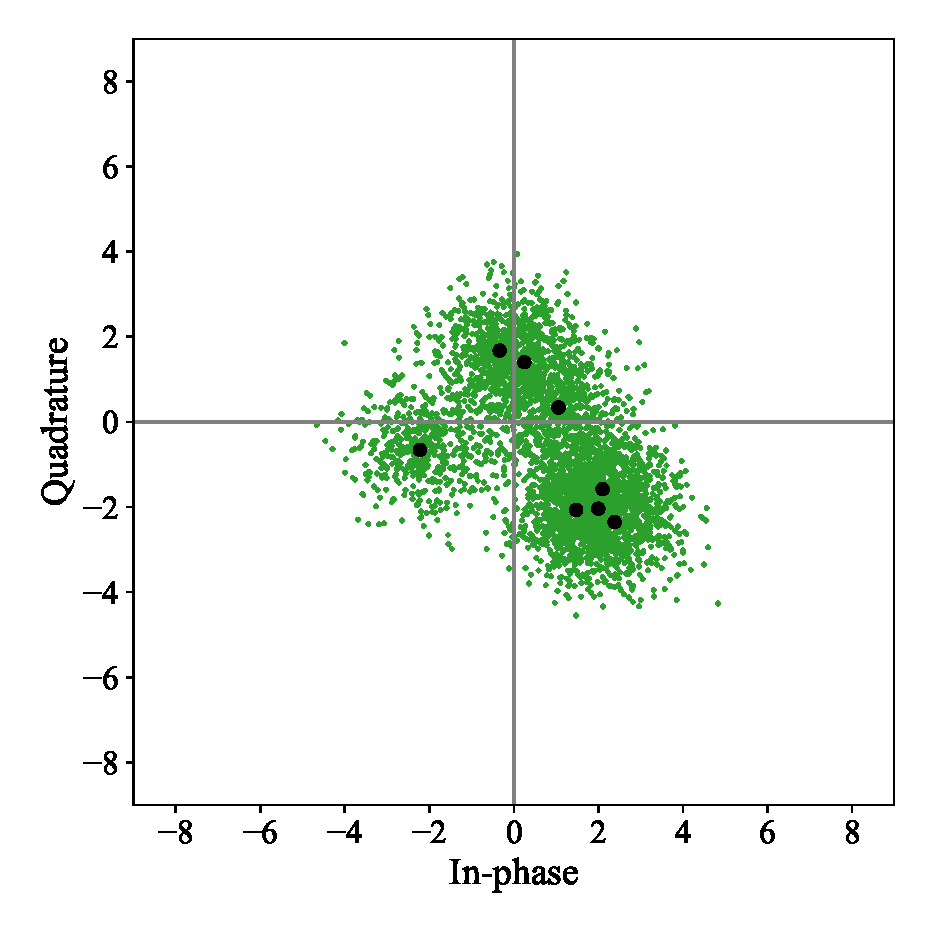
\includegraphics[width=\linewidth]{figs/awgn_normal_constellation}
		\caption{With no covert transmission}
	\end{subfigure}
	\hfill
	\begin{subfigure}{0.24\textwidth}
		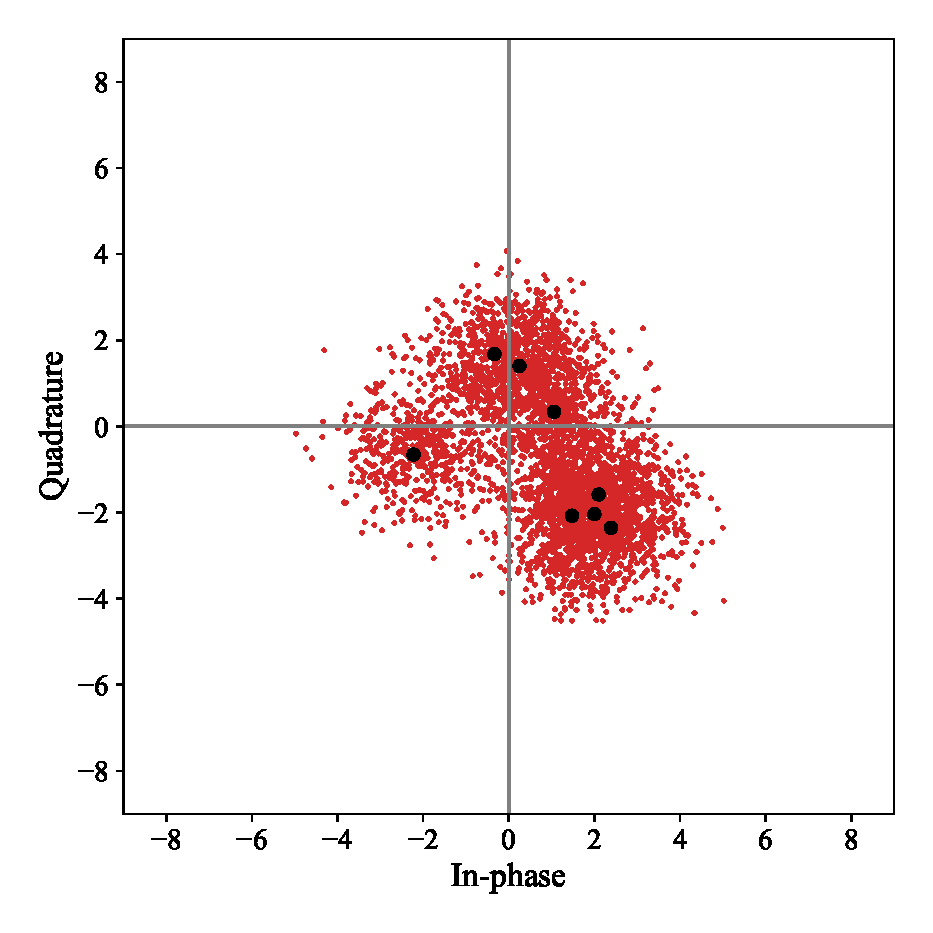
\includegraphics[width=\linewidth]{figs/awgn_covert_constellation}
		\caption{With covert transmission}	
	\end{subfigure}
	\caption{Comparing constellation clouds of a signal before and after our covert scheme being applied on the AWGN channel.}
	\label{fig:awgn_constellation}
\end{figure}
\begin{figure}[tp!]
	\begin{subfigure}{0.24\textwidth}
		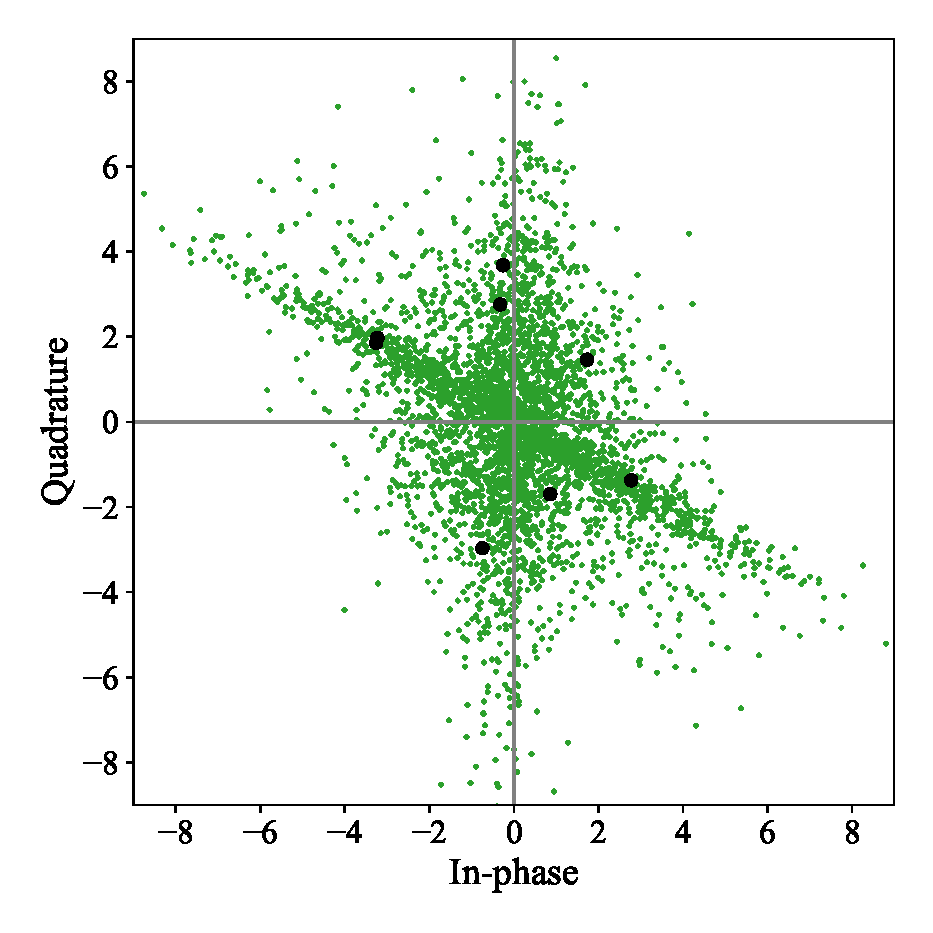
\includegraphics[width=\linewidth]{figs/rayleigh_normal_constellation}
		\caption{With no covert transmission}
	\end{subfigure}
	\hfill
	\begin{subfigure}{0.24\textwidth}
		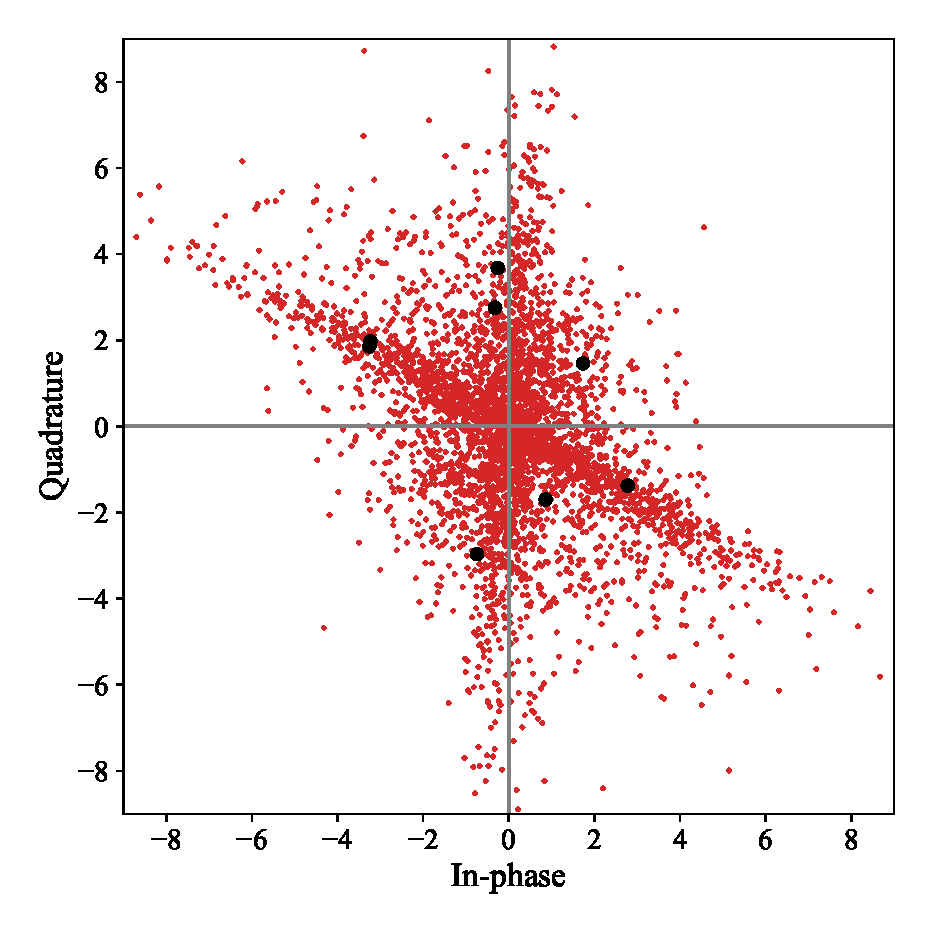
\includegraphics[width=\linewidth]{figs/rayleigh_covert_constellation}
		\caption{With covert transmission}	
	\end{subfigure}
	\caption{Comparing constellation clouds of a signal before and after our covert scheme being applied on the Rayleigh fading channel.}
	\label{fig:rayleigh_constellation}
\end{figure}
